%% A simple template for a lab or course report using the Hagenberg setup
%% with the standard LaTeX 'report' class
%% äöüÄÖÜß  <-- keine deutschen Umlaute hier? UTF-faehigen Editor verwenden!

\documentclass[a4paper,english,11pt]{report}		
%\documentclass[a4paper,ngerman,11pt]{report}

\usepackage{hgb}
\usepackage{hgbabbrev}
\usepackage{hgblistings}
\usepackage{hgbbib}
\usepackage{hgbheadings}
\usepackage{mathtools}

\RequirePackage[utf8]{inputenc}		% remove when using lualatex oder xelatex!

\graphicspath{{images/}}  % where are the images?
\bibliography{references}  % requires file 'references.bib'

\author{Anna M.\ Maureder}
\title{Unsupervised identification of the rigid part of an unknown articulated object}
\date{\today}

%%%----------------------------------------------------------
\begin{document}
%%%----------------------------------------------------------
\maketitle
\tableofcontents
%%%----------------------------------------------------------

\chapter {Pose estimation}

\section{Initial idea}

The initial project idea was to create a tool for 3D animation purposes using a small puppet to capture its poses in real-time. However, the idea addressed many different challenges, like 3D reconstruction, segementation, joint and skeleton estimation as well as creating a interface with a 3D animation program. As the implementation of these tasks would go beyond the scope of a thesis project, it was indispensible to break it down into its main areas. While doing researches on pose estimation, the issue of segmenting an articulated object into its rigid part frequently emerged and for this reason the thesis project will focus on this field.

\section{Motivation}

Pose and motion estimation of objects is an active field of research due to the growing digitalization of day-to-day processes. A vast majority of existing pose estimation methods take advantage of sensors and markers as an indicator for the joints of an object. Additionaly, the rigid parts and of an object and its joints are already known. However, unsupervised methods that are completly independent of user input and detect the pose of an unknown object, constitute a great challenge. Among those methods, the non-rigid registration is a well-known approach \cite{survey}.

\section{Related Work}
\label{cha:relatedWork}

An overview of related methods to non-rigid registration for detecting rigid body parts of an articulated object are mentioned by Chang \cite{chang08articulated} and Tam  which mainly use the ICP (iterative closest point) and the PCA (Principal component analysis) to find corresponding body parts. This paper is based on the Correlated Correspondance algorithm \cite{CorrelatedCorrespondance} \cite{Anguelov04} and Symmetrization \cite{Mitra07}. A following work to \cite{chang08articulated} is \cite{chang09range}. Other methods include temporal coherence, markers and user inputs. Another method handels the registration process by first detecting the largest rigid part \cite{correspondence}.

\subsection{EM-algorithm}

Here comes an explanation of Anguelov with pictures.

\subsection{LRP}

Here comes the LRP algorithm with pictures.

\subsection{Symmetrization}

Here comes an explanation of symmetrization.

\chapter{My contribution}
\label{cha:MyContribution}

This chapter focuses on the implementation of a new segmentation approach by taking the existing methods as reference (see section \ref{cha:relatedWork}). The algorithm has been first implemented in 2D, in order to be able to focus solely on developing and testing. Subsequently, it will be implemented in 3D using the PCL.

\section{Goal and approach}

The goal is to segment an articulated mesh $M$ into its unknown number $n$ of rigid parts $ P =  \{ {p_1,....p_n}\}$ and extract the joints $ J =  \{ {j_1,....j_{n-1}}\}$ linking those parts in form of a skeleton structure. In general, this is done by non-rigid registration of the point clouds $S\textsubscript{0}$ and $D\textsubscript{0}$ of an object in two different poses. $S_0$ is thereby used as a \textit{template} to be registered with $D_0$. The main task is to determine a part assignment $p_i$ and the corresponding transformation $t_i$ for all points of the \textit{template} that alligns them with all points of $D_0$. Basically, a divide and conquer approach (see section \ref{divideAndConquer}) is implemented to recursively subdivide $S_0$ and $D_0$ into clusters trying to be matched.

\section{Assumptions}

The input mesh $M$ is assumed to solely consist of rigid parts that can not be deformed or stretched (e.g. rigid parts of a human) and are linked by joints. Comparing two poses $S_0$ and $D_0$ being adopted by the articulated object, the geodesic distance $g_{i,j}$ between two mesh points $p_i$ and $p_j$ remains constant. Thereby, it is taken advantage of the knowledge that points located on a rigid part $p_i$ have the same transformation $t_i$ . Furthermore, it is assumed that the two poses $S_0$ and $D_0$ of $M$ are oriented in the same direction.

\section{Challenges/restrictions}

There are many challenges regarding the non-rigid registration of point clouds in 2D, as well as in 3D. First off, the input data can be noisy by means of points not belonging to the object. Furthermore, the approach is computationally expensive and time-consuming, as the corresponding body parts of two meshes need to be detected iteratively. Additionally, the inevitable difficulty of finding the global optimum, related to ambiguous body parts, has to be overcome.

\section{Approach}
\label{divideAndConquer}

\subsection{General idea}

The algorithm starts with two sets of point clouds $S_0$ and $D_0$ of an object $M$ in different poses (see figure \ref{fig:dc_original_p2}). The two point clouds are iteratively subdivided into point clusters $ C =  \{ {c_1, ... , c_m}\}$. In each iteration step two related clusters of $S_0$ and $D_0$ are matched by applying the ICP (iterative closest point) resulting in a matching error $e$. In case of $ e < \tau $, two clusters are assumed to match. Otherwise, the algorithm is applied recursively and the clusters are again subdivided into further clusters. The algorithm terminates if all resulting clusters of $S_0$ can be matched to all clusters of $D_0$. All neighboring clusters are then checked to be merged, in case of having divided a rigid part. After that step, the remaining clusters are assigned to rigid parts $ P =  \{ {p_1, ..., p_n}\}$.

\begin{figure}
	\centering
	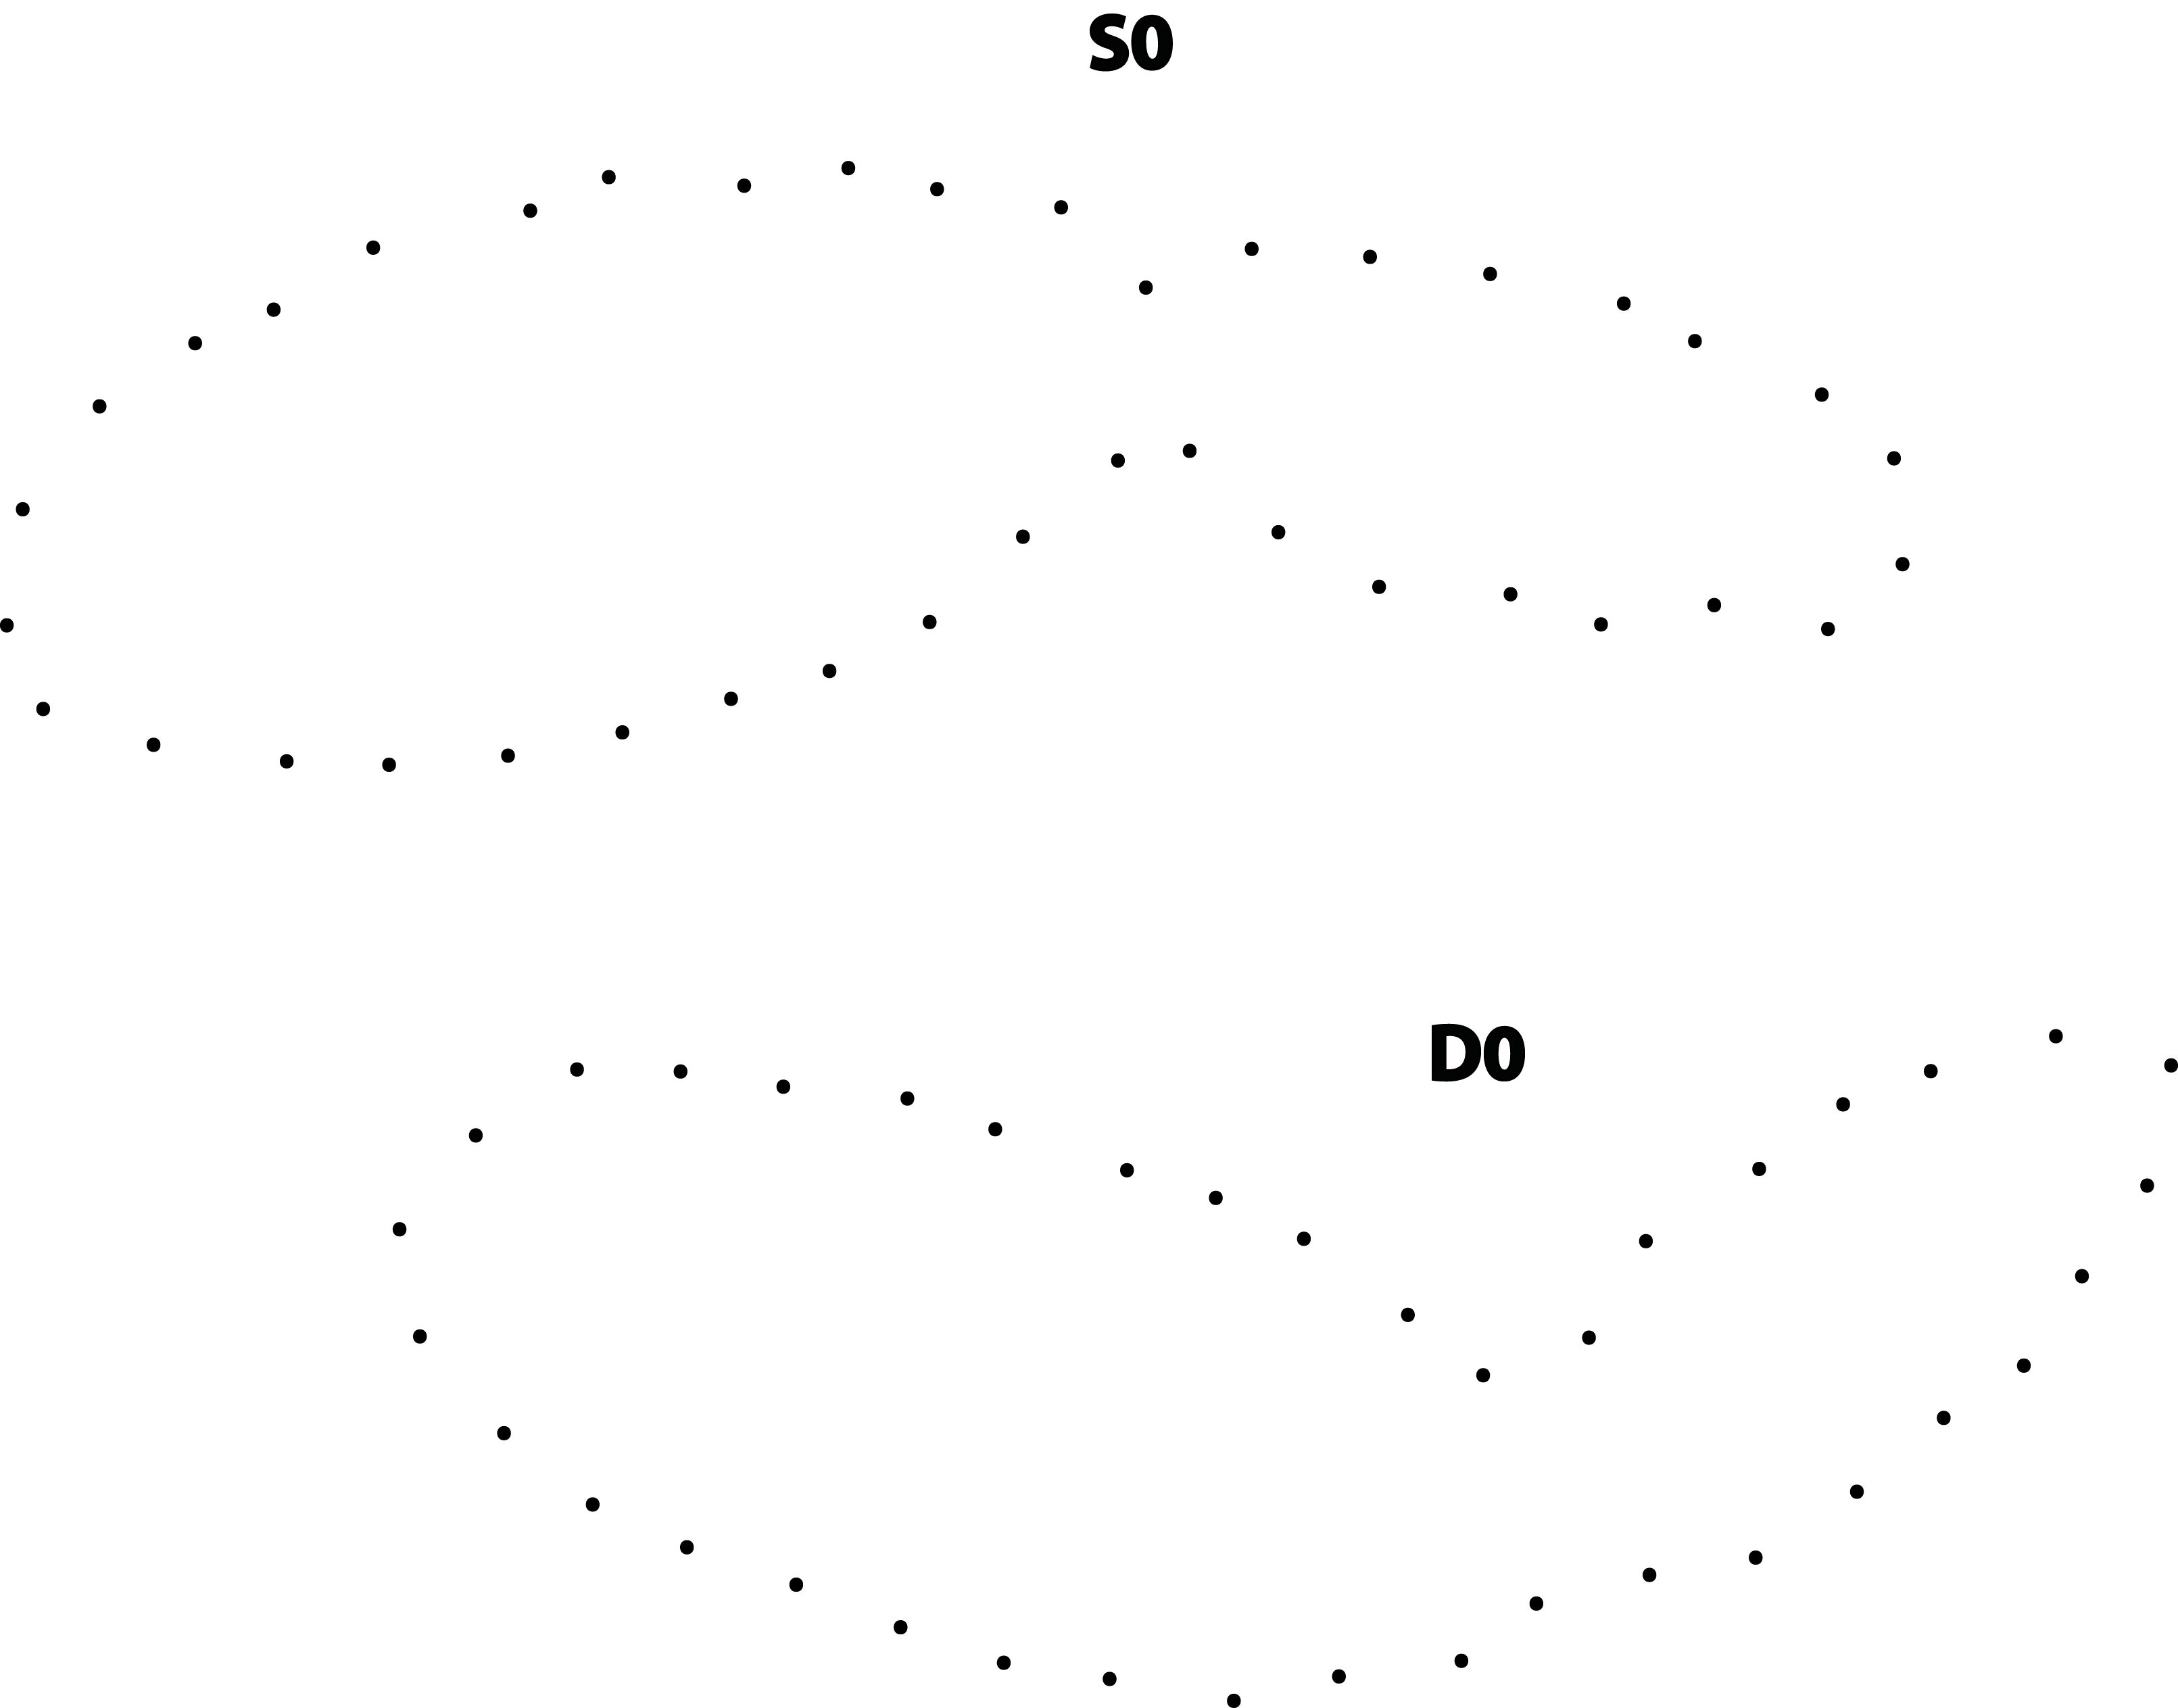
\includegraphics[width=0.7\linewidth]{illustration_original}
	\caption{Taking a mesh \textit{M} in two different poses \textit{S\textsubscript{0}} and \textit{D\textsubscript{0}} as input.}
	\label{fig:dc_original_p2}
\end{figure}

\subsection{Removing outliers}

As a first step, the outliers of the two point clouds $S_0$ and $D_0$ are removed. This is done, by detecting point clusters $C = \{{c_0, ... , c_m}\}$. A cluster $c_i$ starts with an unclustered point $p_i$ of $S_0$ or $D_0$. Another point $p_j$ is then added to the cluster $c_i$ if the euclidean distance between them $d_e(p_i, p_j)$ is under a certain threshold $\tau$. If $p_j$ can not be assigned to any cluster of $C$ a new cluster $c_{m+1}$ is created. Once all points of $S_0$ and $D_0$ are assigned to clusters, the biggest cluster $c_0$ is selected.

\subsection{Subdividing into clusters}

As a next step, the two main clusters $c_0$ are taken as input for further computation steps. If the matching between the two clusters does not suceed, they are subdivided into two clusters. In the other case, no subdividing is done and the procedure is repeated recursively for all clusters $C = \{{c_1, ..., c_m}\} $ of $S_0$ until they can be matched to all clusters of $D_0$.   

\subsubsection{Divider position}

To determine where to divide a cluster, it is taken advantage of the PCA (principal component analysis). The resulting dividers $d_S$ and $d_D$ are realised by computing the principal axes $p_S$ and $p_D$ through the centroids $ct_0$ and taking the perpendicular secondary axes $s_S$ and $s_D$ through the centroids (see figure \ref{fig:dc_axes_2p}).

\begin{figure}
	\centering
	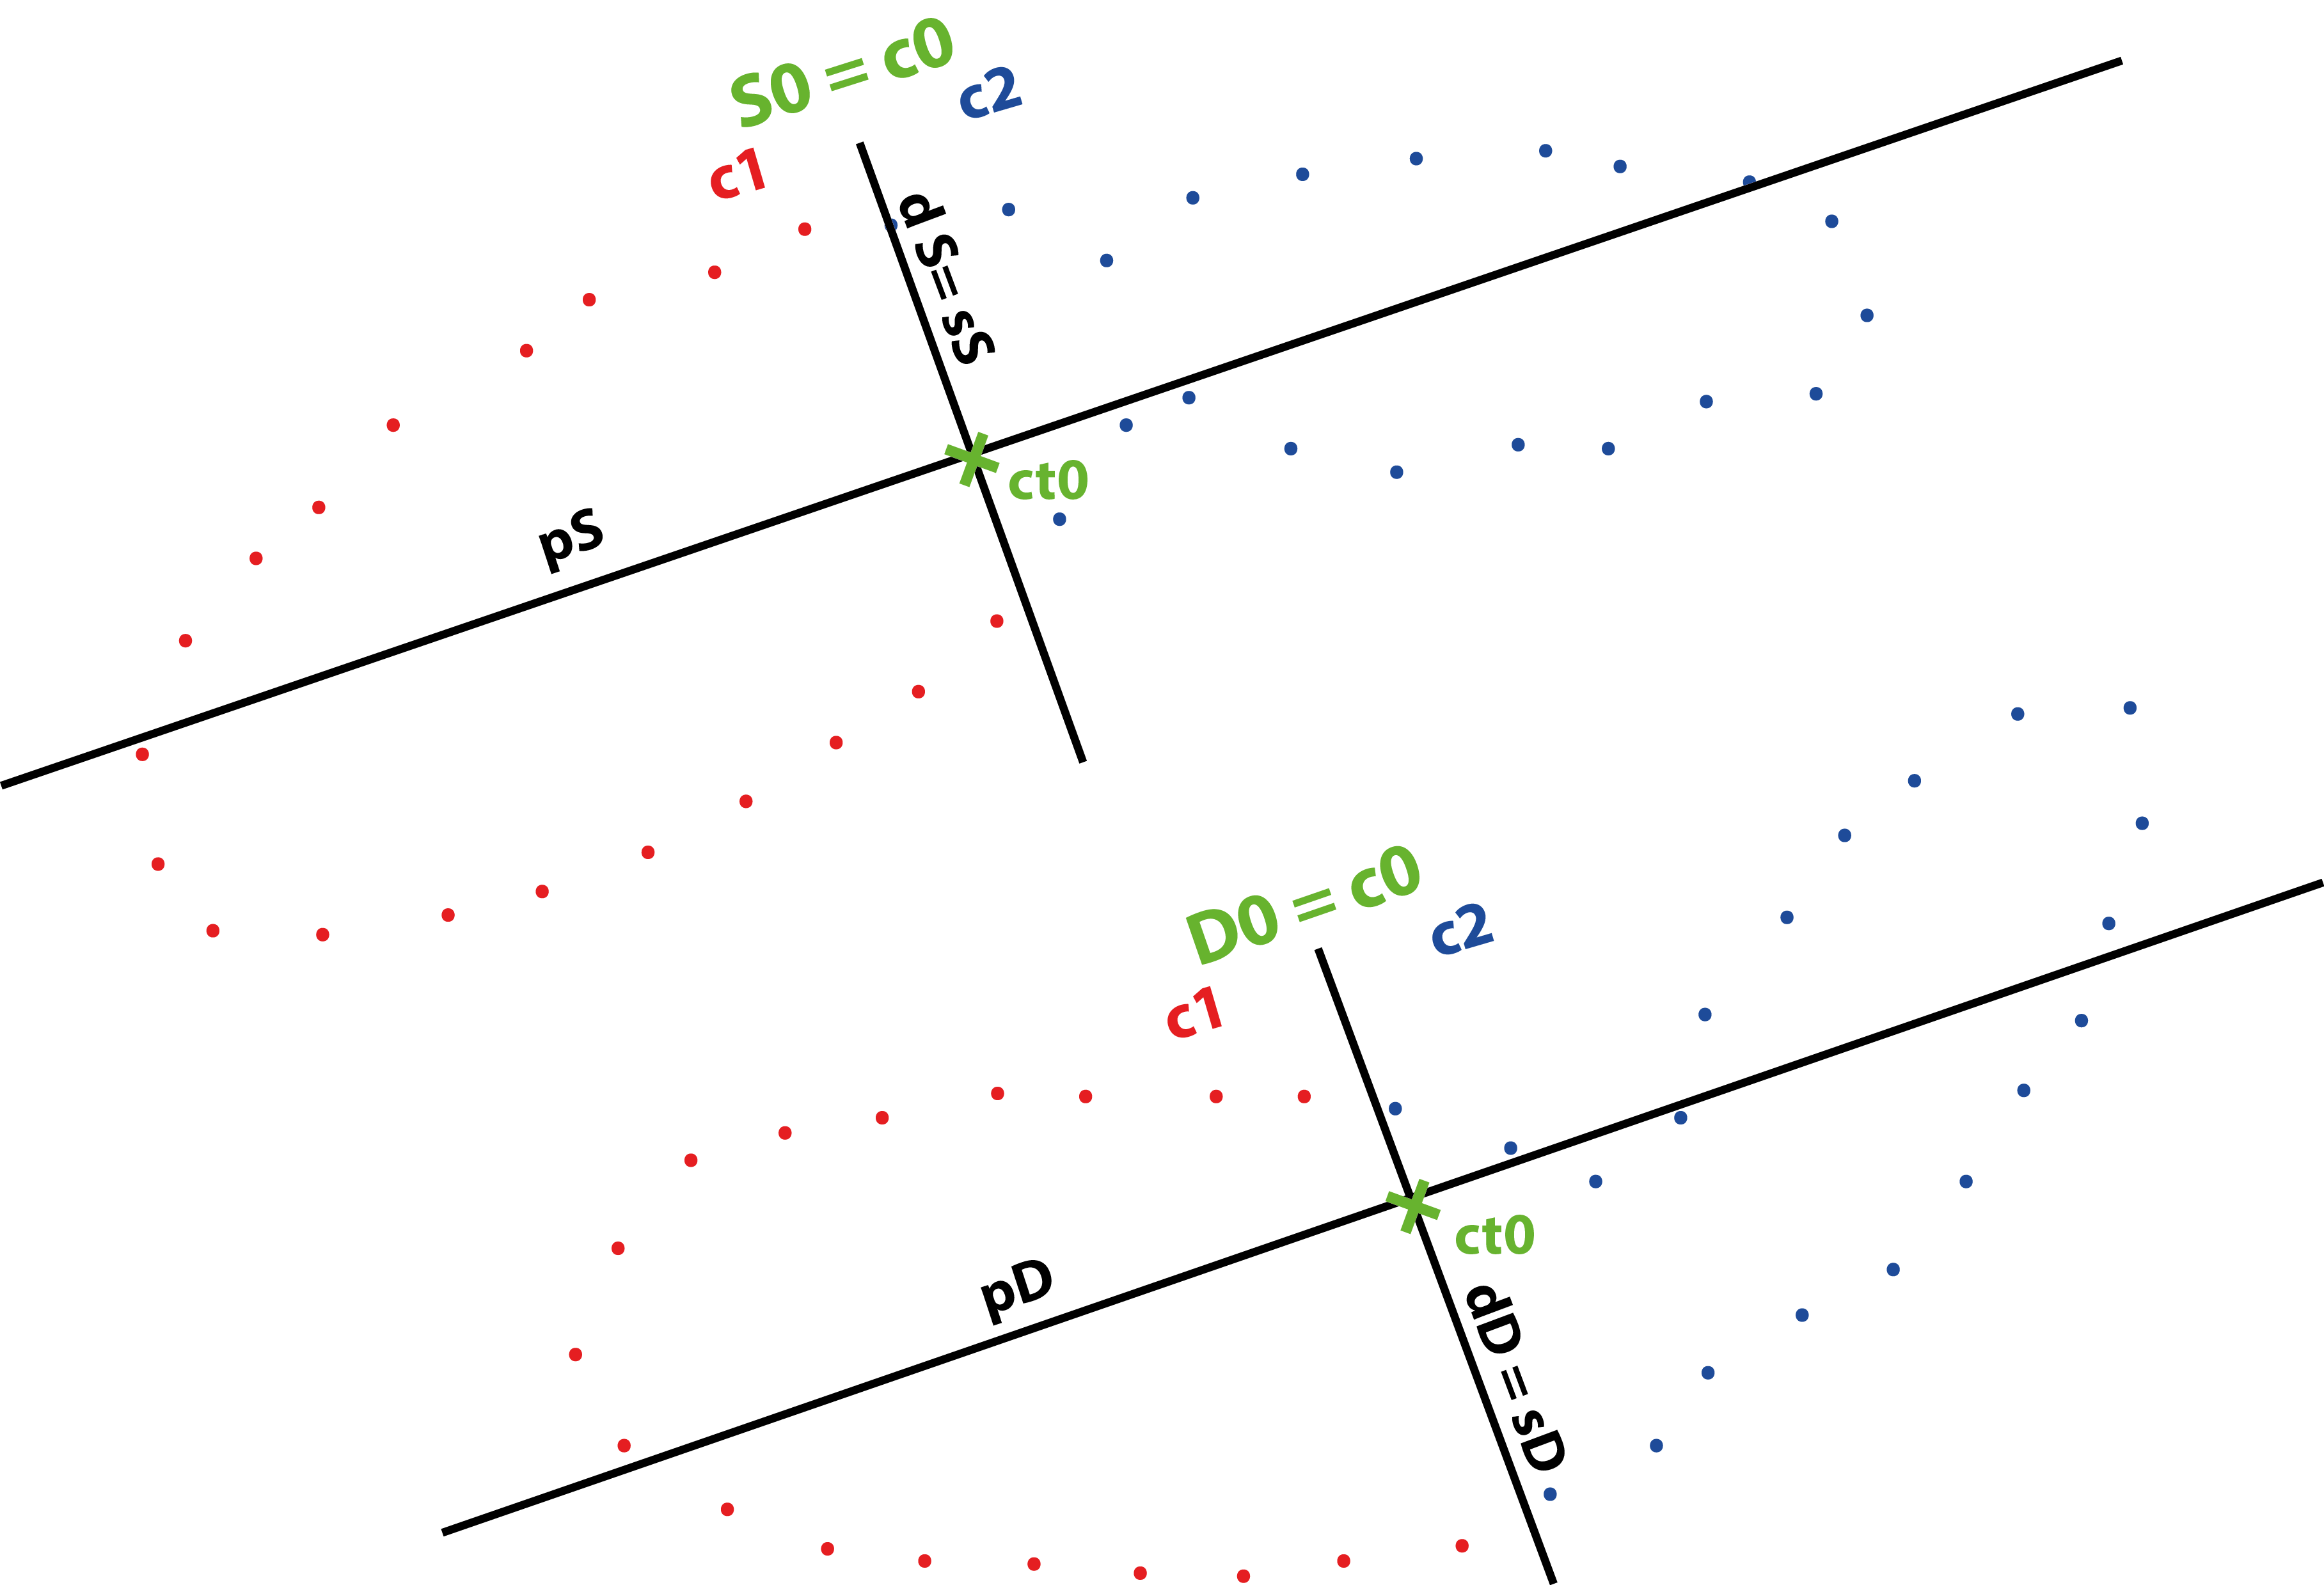
\includegraphics[width=0.7\linewidth]{illustration_axes}
	\caption{Dividing \textit{S\textsubscript{0}} and \textit{D\textsubscript{0}} into clusters by the divider \textit{d} to match them with ICP.}
	\label{fig:dc_axes_2p}
\end{figure}

\subsubsection{Declaring the matching condition between two clusters}

By applying the ICP and the nearest neighbour approach on two associated clusters $c_i$ of $S_0$ and $D_0$, a certain matching error is computed between the cluster points
$ CP =  \{ {cp_0, ..., cp_n}\}$ and the associated points $ QP =  \{ {qp_0, ..., qp_n}\}$. To declare when two clusters are matching, it is important to find an appropriate threshold $\tau$. In case of being overvalued, clusters are more likely to be matched which could result in insufficient subdividing. On the other hand, the clusters are difficult to be matched, which will result in further subdividing and too many rigid parts. To make the matching error independent of the amount of cluster points, an average error per point
%
\begin{equation}
e_{avg} = \frac{\displaystyle\sum_{i=0}^{m}\| cp_i - cq_i\|^2}{| CP |}
\end{equation}
%
is computed, assuming that the two clusters $c_{S, i}$ and $c_{D, i}$ contain the same amount of cluster points $m$. In case of different point amounts, the segmentation needs to be carried out at that clusters are always the same amount of points or some points are not considered during error amount calculation.

Version 1:



Version 2:

\subsubsection{Cluster tree}
\label{tree}

The subdividing of the clusters $c_0$ is realised by a depth-first approach in a binary tree. Consequently, $S_0$ and $D_0$ are subdivided from the left to the right. A node $N$ of the tree contains two related clusters $c_i$ of $S_0$ and $D_0$ and in case of subdividing it, a Node \textit{left} and \textit{right}, containing the subdivided clusters $c_{i+1}$ and $c_{i+2}$. If two associated clusters in a Node $n_i$ match, no further subdividing is performed. The resulting leaves of the three are stored as matching clusters $C_l = \{{c_{l1}, ... , c_{lm}}\}$ (see figure \ref{fig:illustrationTree}). By applying the depth-first approach, the neighboring clusters in the list are also neighbouring clusters in the object $S_0$ or $D_0$.  As a result, in the following steps the skeleton structure from an object can be extracted, where parts are connected by joints.

\begin{figure}
	\centering
	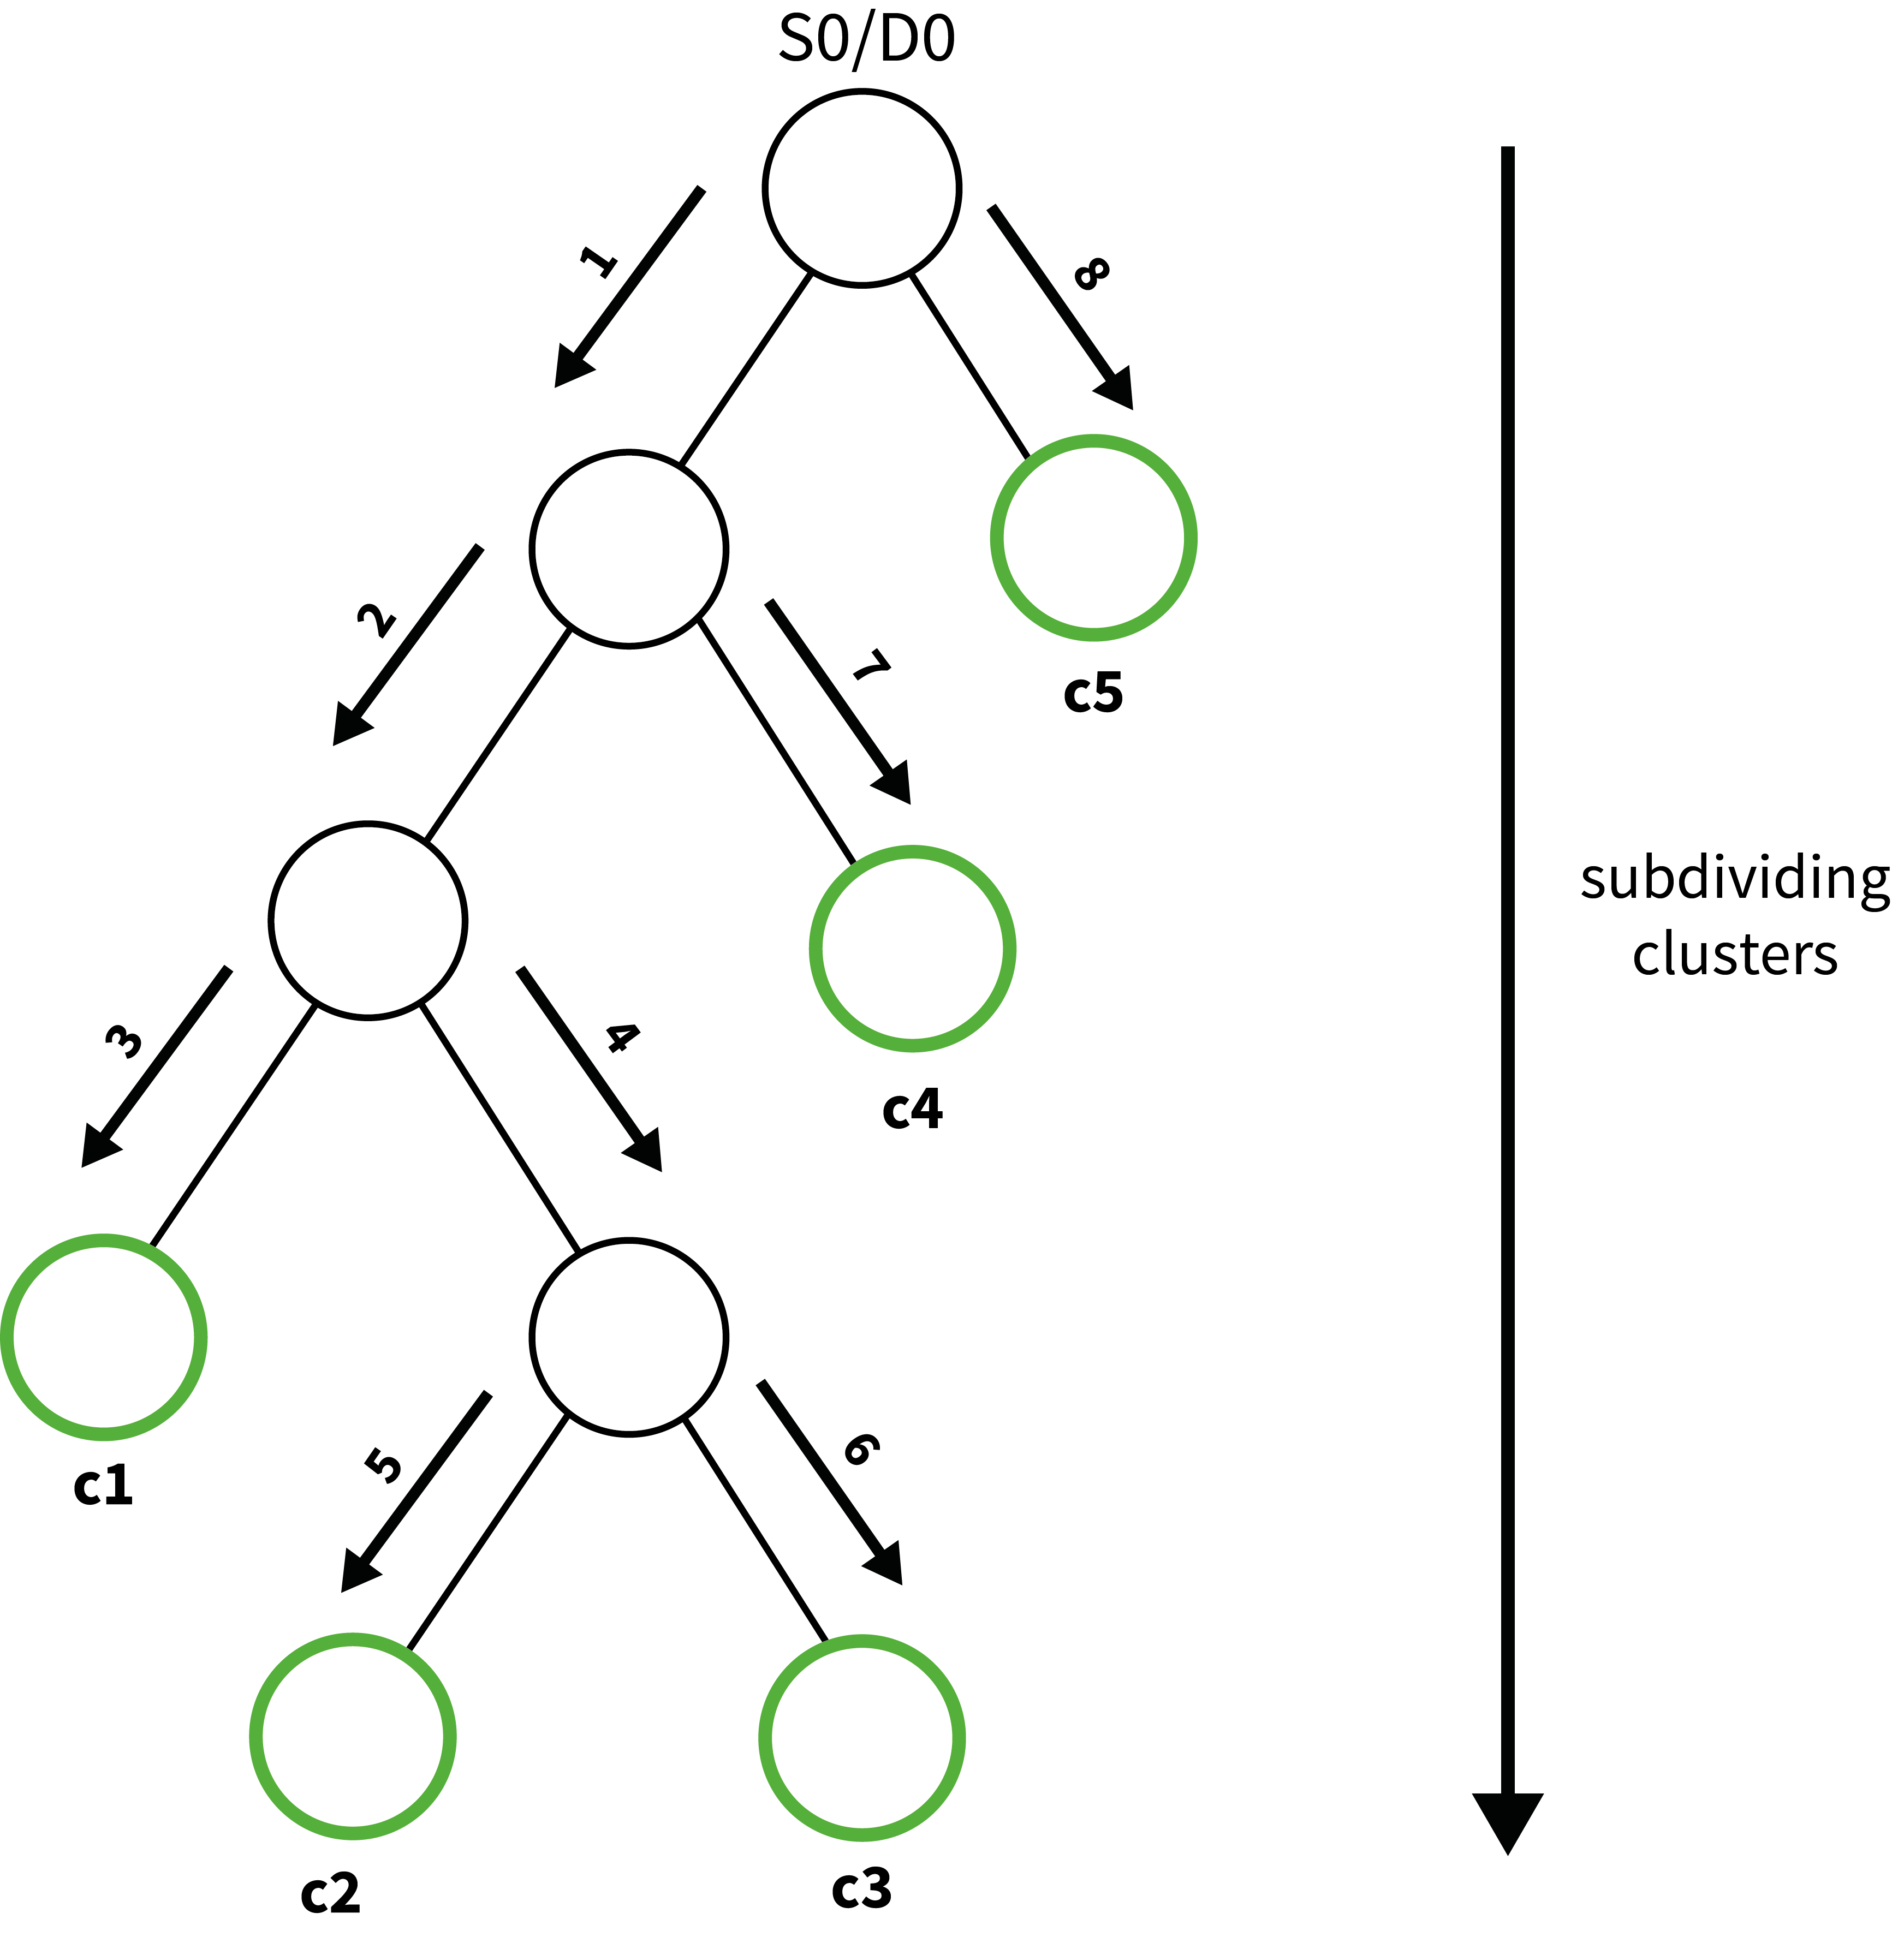
\includegraphics[width=0.7\linewidth]{IllustrationTree}
	\caption{Subdividing of S0 and D0 into matching clusters by the depth-first approach}
	\label{fig:illustrationTree}
\end{figure}

\subsection{Merging neighboring clusters to rigid parts}

As a next step, neighboring clusters from $C_l$ are iteratively merged and subsequently verified to match. This process is required to rejoin, if necessary, detected sub clusters to the rigid parts of the object. This is the case, if during the subdividing process, a rigid part was subdivided. The merging initiates with the first cluster $c_{li} = c_{l1}$ and its adjacent cluster $c_{li+1}$. If the resulting merged clusters $c_{ri} = c_{r1}$ can be matched, the merging proceeds with $c_{ri}$ and the adjacent cluster $c_{li+2}$. If not, the merging is not executed and $c_{li}$ is stored in a list of resulting clusters $C_r$. The whole procedure then starts with $c_{li+1}$. The process terminates if all clusters of $C_l$ are verified and consequently the clusters of $C_r$ are assigned to rigid parts $ P =  \{ {p_1,....p_n}\}$ (see figure \ref{fig:clusterChain}). 

\begin{figure}
	\centering
	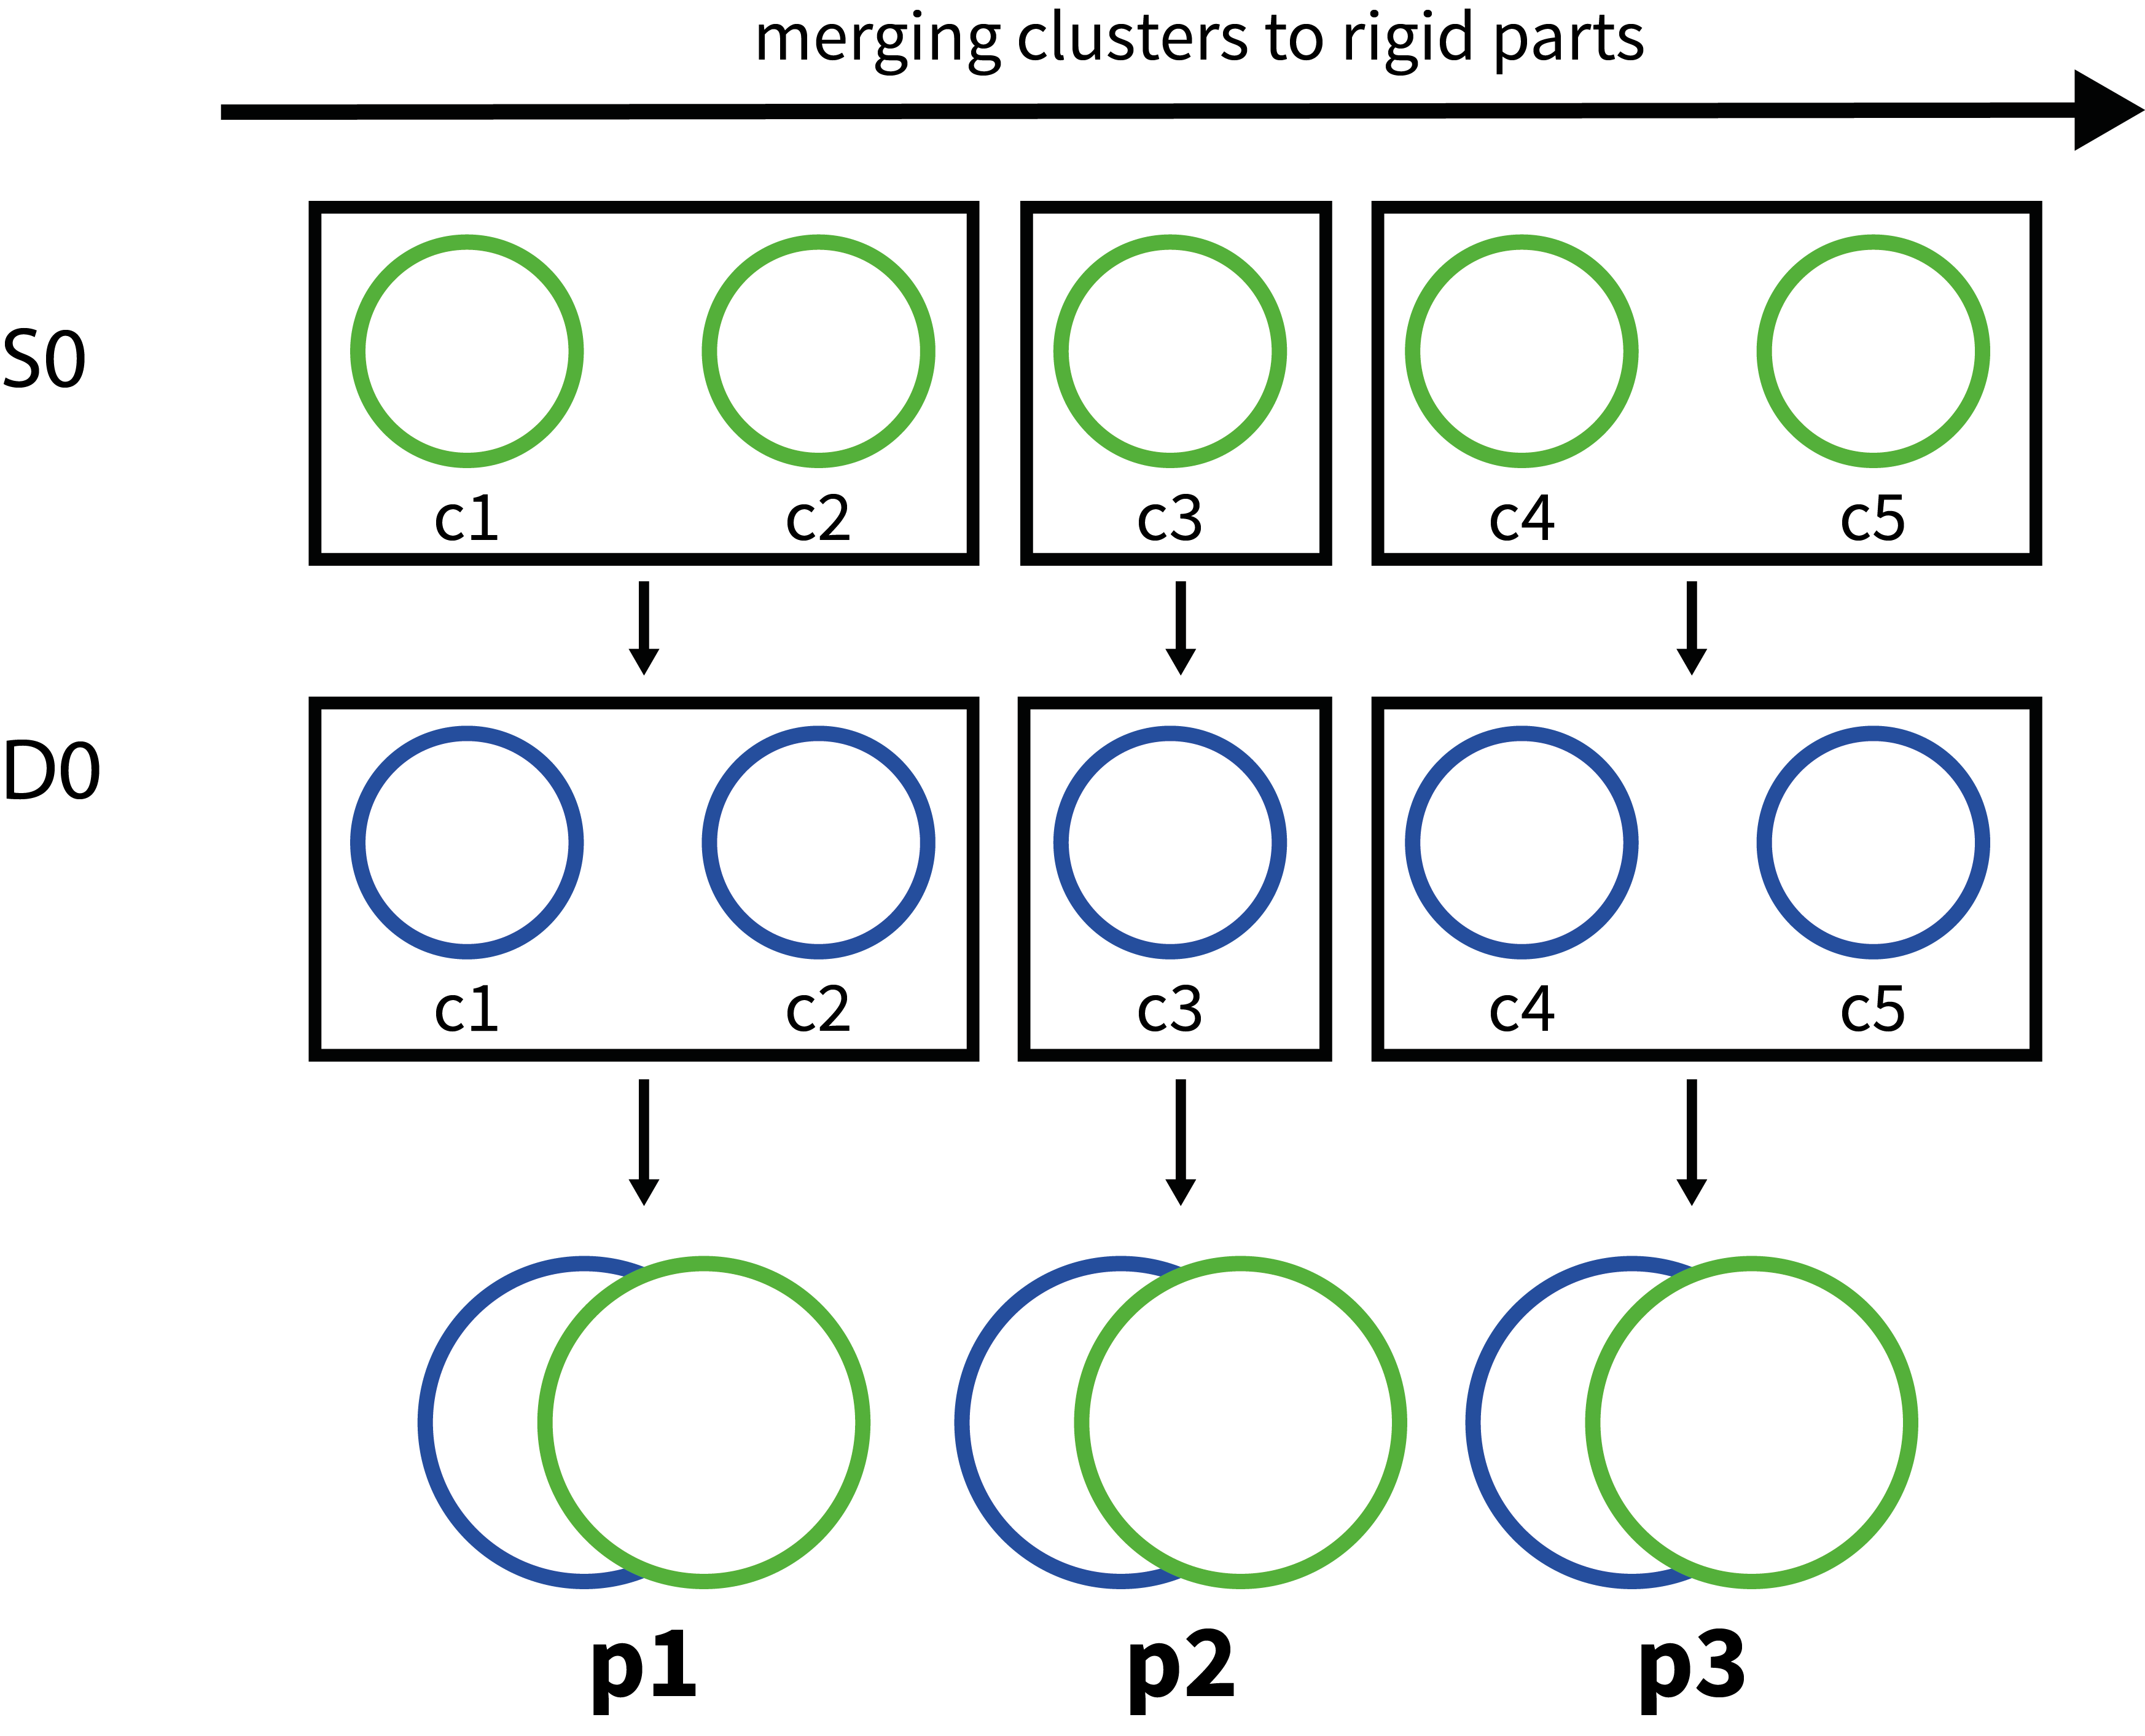
\includegraphics[width=0.7\linewidth]{ClusterChain}
	\caption{Detecting rigid parts of S0 and D0 by iteratively merging neighboring clusters of S0 and matching them with the merged clusters of DO.}
	\label{fig:clusterChain}
\end{figure}

\subsection{Joint/skeleton estimation}

After detecting the rigid parts $ P =  \{ {p_1,....p_n}\}$, they are linked with joints and the principal axes are for now assumed to form the skeleton. 

\section{Implementation}

My approach was implemented in Java, using ImageJ as processing library, to focus on implementing and testing the algorithm in 2D. Another implementation is planned for 3D with the PCL to bring the attention to segmentation in 3D, and visualization. A class Cluster was implemented to store cluster points, the centroid, the orientation as well as the principal and secondary axes. For the subdividing, a cluster tree was implemented to simultainiously divide the initial clusters $c_{S, 0}$ and $c_{D, 0}$ into sub clusters. Each node $N$ contains thereby two associated clusters $c_{S, i}$ and $c_{D, i}$. For the clustering and merging of clusters a List of Clusters was used to dynamically add/remove Clusters. Furthermore, a class ICP was created, which takes two clusters to be matched as input.

\subsection{Implementation Steps}

\begin{enumerate}
	\item The point clouds $S_0$ and $D_0$ are taken as input and clustering is computed to get the biggest clusters $c_{S, i}$ = $c_{S, 0}$ and $c_{D, i}$ = $c_{D, 0}$.
	
	\item The centroids $ct_{S, i}$ and $ct_{D, i}$ of $c_{S, i}$ and $c_{D, i}$ are computed.
	
	\item The principal axis $p_{S, i}$ and $p_{D, i}$ are computed through $ct_{S, i}$ and $ct_{D, i}$ in order to orient and align $c_{S, i}$ and $c_{D, i}$.
	
	\item The secondary axis $s_{S, i}$ and $s_{D, i}$ perpendicular to $p_{S, i}$ and $p_{D, i}$ through $ct_{S, i}$ and $ct_{D, i}$ are computed.
	
	\item The ICP between $c_{S, i}$ and $c_{D, i}$ and an error distance per point $e_{avg}$ are computed. 
	
	\item In case of $e_{avg} > \tau$, the dividers $d_{S, i}$ and $d_{D, i}$ to subdivide $c_{S, i}$ and $c_{S, i}$ are initialized with the secondary axis $s_{S, i}$ and $s_{D, i}$.
	
	\item The cluster points $ CP =  \{ {cp_0, ..., cp_n}\}$ of $c_{S, 0}$ and $c_{D, 0}$  are either allocated to $c_{S, i + 1}$ or $c_{S, i + 2}$ depending on its position $cp_i.x$ to $ct_{S, i}.x$ and $ct_{D, i}.x$. 
	
	\item The algorithm continues with $c_{S, i}$ = $c_{S, i + 1}$ from step 2.
	
	\item If $e_{avg} \le \tau$
	
	\item An error distance \textit{e\textsubscript{left}} and \textit{e\textsubscript{right}} is obtained. The part with the most error per point is assumed to be not rigid which gives back an indicator where to divide \textit{S\textsubscript{0}} and \textit{D\textsubscript{0}}.
	
	\item The dividers \textit{d\textsubscript{S}} and \textit{d\textsubscript{D}} are shifted to the direction of the highest error. To be continued from step 5 until the total error \textit{e\textsubscript{total}} doesn't get smaller.
\end{enumerate}

\subsection{Intermediate results}

First on, the implementation was tested with two point clouds of an articulated object with only two rigid parts. Figure XX shows the clusters of the object after subdividing, figure XX shows the resulting rigid parts. The results are directly dependent of error threshold $\tau$. In case of XXX too many segments are detected, in case of XXX no segmentation is conducted. (see Figure \ref{fig:dc_results_2p}). 

\begin{figure}
	\centering
	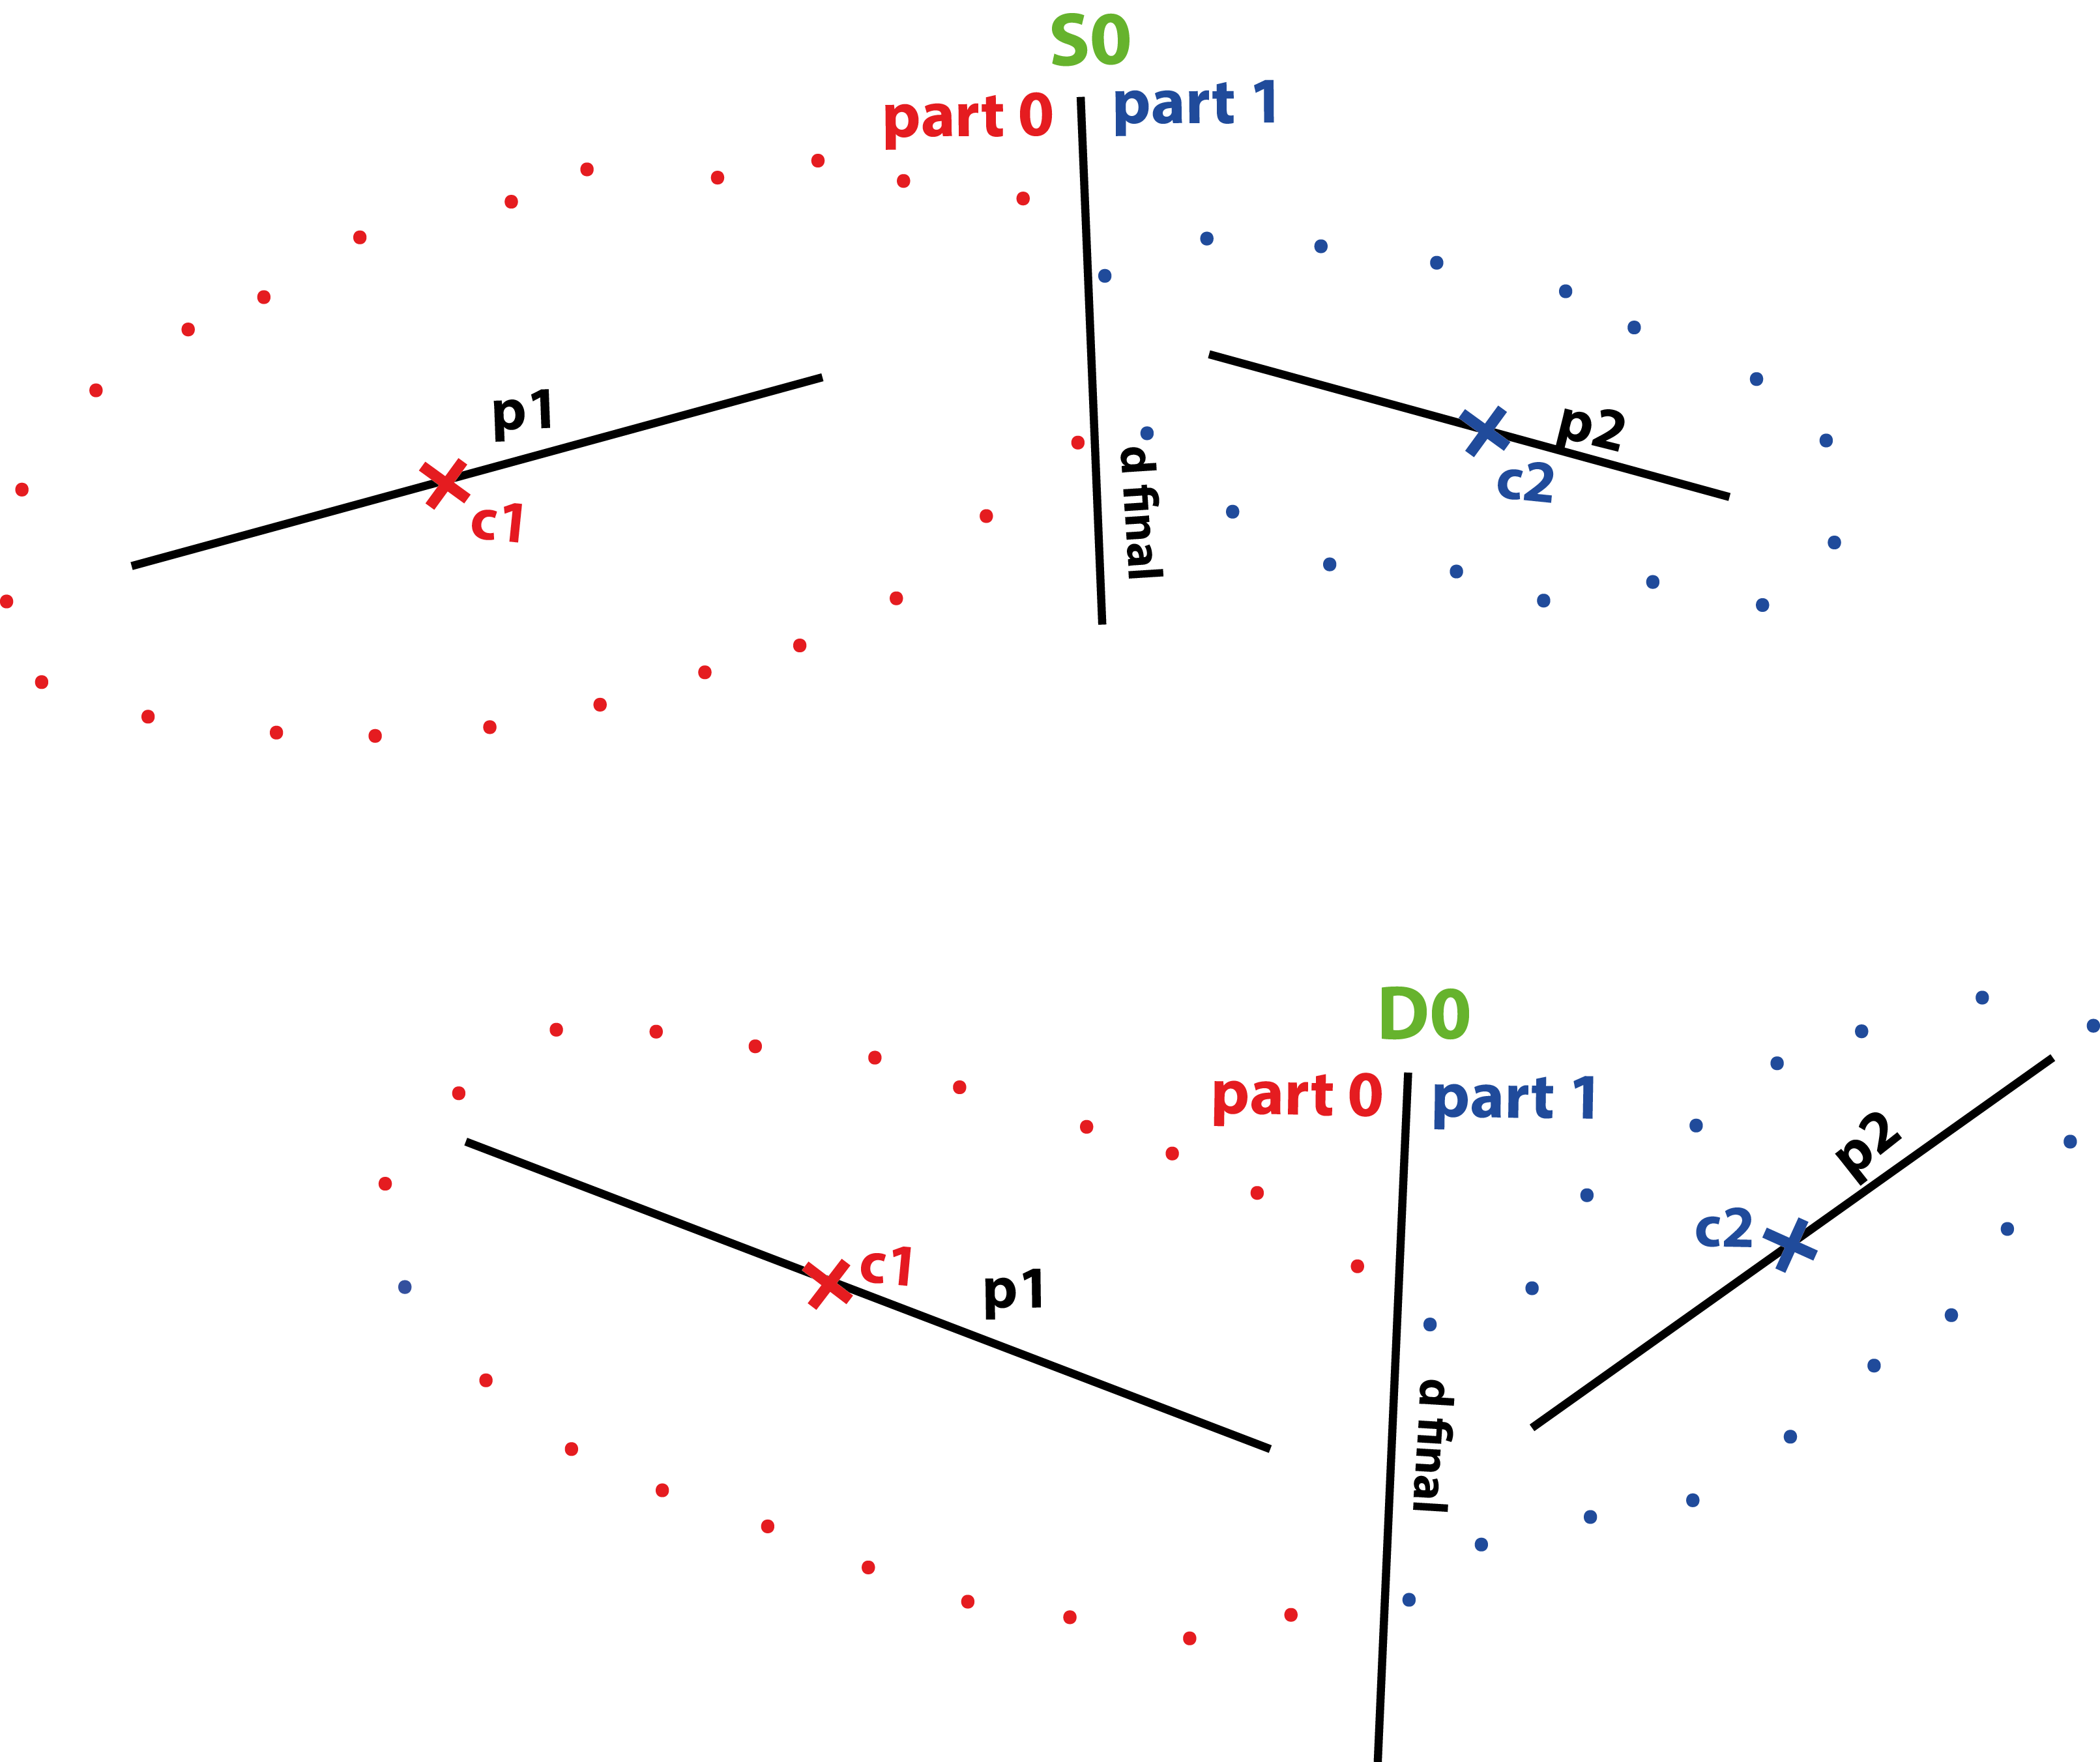
\includegraphics[width=0.7\linewidth]{illustration_results}
	\caption{Assigning of the rigid parts \textit{P =(part\textsubscript{0}, part\textsubscript{1})} after termination of segmentation process.}
	\label{fig:dc_results_2p}
\end{figure}


Results from easy examples. Not working for human, as by dividing of one cluster, breaking down into single clusters (see Figure X). Another approach, e.g. using LRP as an initial alignment to then recursively segment the clusters linked to the LRP. Clusters not matching, as they don't have the same number of points, each point can only have one neighboring point. Or dividing clusters that they all have the same amount of points. In case of a more complex object where one rigid part can be linked with a high number of rigid parts (upper body of a humen) another approach has to be found, as the skeleton structure is different than from a chain. (see Figure \ref{fig:dc_results_2p}).

\subsection{Possible Improvements}


\subsubsection{LRP as initial alignment}

As only objects with rigid parts arranged like a chain are possible with this approach, another improvement/algorithm has to be pursued (see section \ref{sec:LRP}).

\section{LRP as initial alignment}
\label{sec:LRP}

Instead of cutting the object initially in half, as an initial step the largest rigid part is found and recursively from there all other linked parts can be detected.

\subsection{Overview}
As an initial step, the LRP algorithm tries to find the most reliable correspondences, the so-called largest rigid part (LRP), subsequently all other parts are detected that are linked to the LRP. The initial alignment stage tries to find sparse correspondences between two point clouds by applying a single rigid transformation to detect the largest subsets of points in two point clouds. Starting from the LRP all other parts are detected recursively.

\subsection{Algorithm} 

\subsubsection{Finding the LRP}

The algorithm also takes two point clouds \textit{S\textsubscript{0}} and \textit{T\textsubscript{0}} of the same object in different configurations as input.
The goal is to find a single rigid transformation \textit{T\textsubscript{init}} for all points of \textit{S\textsubscript{0}} to get potential corresponding points \textit{C\textsubscript{0} = \{(s\textsubscript{i}, t\textsubscript{j})\}} in \textit{T\textsubscript{0}}. For that, local descriptors of \textit{S\textsubscript{0}} and \textit{T\textsubscript{0}} are computed. The requirement for a sparse correspondance between two points \textit{s\textsubscript{i}} and \textit{t\textsubscript{j}}  is that they are \textit{reciprocal}, which means that the Euclidean distance \textit{d(s\textsubscript{i}, t\textsubscript{j})} between them is the smallest in both directions. Some of the sparse correspondances are asumed to be wrong. Therefore, RANSAC is used on the sparse correspondances \textit{C\textsubscript{0}} to estimate a rigid alignment that is supported by the largest number of points \textit{n} from \textit{S\textsubscript{0}} and \textit{T\textsubscript{0}}. To assign the LRP in \textit{S\textsubscript{0}} and \textit{T\textsubscript{0}}, the biggest point clusters \textit{C\textsubscript{s}} and \textit{C\textsubscript{t}} of the overlapping area \textit{G\textsubscript{s} = \{C\textsubscript{1}, ... , C\textsubscript{n}\} } and \textit{G\textsubscript{t} = \{C\textsubscript{1}, ... , C\textsubscript{n}\} } are detected. 


\subsubsection{Part discovery}

The remaining clusters from \textit{S\textsubscript{0}} and \textit{T\textsubscript{0}} that have not been registered yet are matched recursively by starting with clusters connected to already matched parts. First, all matched parts are excluded from the input point clouds  \textit{G\textsubscript{s(l+1)}} = \textit{S\textsubscript{0}} - \textit{C\textsubscript{sl}} and \textit{G\textsubscript{t(l+1)}} = \textit{T\textsubscript{0}} - \textit{C\textsubscript{tl}} defining \textit{l} as the number of already matched parts \{1, ..., n\}, \textit{C\textsubscript{sl}}. For that clusters are formed, using region taking into account that they are attached to already registered parts. The algorithm explained is applied until all body parts have been discovered.

\subsection{Steps}

\begin{enumerate}
	\item The centroids \textit{c\textsubscript{s}} and \textit{c\textsubscript{t}} of \textit{S\textsubscript{0}} and \textit{T\textsubscript{0}} are computed.
	
	\item The principal axis \textit{p\textsubscript{s}} and \textit{p\textsubscript{t}}  are computed through \textit{c\textsubscript{s}} and \textit{c\textsubscript{t}} in order to horizontally orient the objects around their centroids.
	
	\item The ICP is conducted as a first guess to find a transformation \textit{T\textsubscript{init}} for all points from \textit{S\textsubscript{0}} that results in the highest number of corresponding points \textit{n} in \textit{T\textsubscript{0}}, given the threshold \textit{T}.
	
	\item \textit{C\textsubscript{0}} contains the corresponding points from S\textsubscript{0} and T\textsubscript{0}, resulting from \textit{T\textsubscript{init}(S\textsubscript{0})}.
	
	\item The RANSAC approach is applied on \textit{C\textsubscript{0}} to find a  \textit{T\textsubscript{f}} that results in the highest number of corresponding points \textit{n} between \textit{T\textsubscript{f}(S\textsubscript{0})} and \textit{T\textsubscript{0}}.
	
	\item The LRP is assigned to \textit{C\textsubscript{s}} and \textit{C\textsubscript{t}} from the resulting point clusters \textit{G\textsubscript{s}} and \textit{G\textsubscript{t}}.
	
	\item Starting from parts that are connected to the LRP, corresponding points \textit{C\textsubscript{i}} for unmatched points from \textit{S\textsubscript{0}} and \textit{T\textsubscript{0}} are seeked. The clusters are given as a input from Step 5. 
	
\end{enumerate}

\section{Other approaches}

\subsection{Points-to-Ellipse fitting}

\subsection{Algorithm}

This algorithm only requires one point cloud containing \textit{m} points \{\textit{pt\textsubscript{0}, ..., pt\textsubscript{m}}\}. The basic idea is to segment the non-rigid object  \textit{S\textsubscript{0}} into its rigid parts \textit{part\textsubscript{1}} and {part\textsubscript{2}} by fitting ellipses to its rigid parts. 
\textit{S\textsubscript{0}} is divided perpendicular to its principal axis \textit{p\textsubscript{0}} into two assumed rigid parts \textit{S\textsubscript{left}} and \textit{S\textsubscript{right}}, initially defining the divider \textit{d} with the secondary axis \textit{s\textsubscript{0}}. The points of \textit{S\textsubscript{left}} and \textit{S\textsubscript{right}} are verified to 
form an ellipse by using its formular

\begin{equation}
\dfrac{x^2}{r_1^2} + \dfrac{y^2}{r_2^2} = 1
\end{equation}

Assuming to verify \textit{S\textsubscript{left}} forming an ellipse, \textit{r\textsubscript{1}} is half the length of the principal axis \textit{p\textsubscript{left}} of \textit{S\textsubscript{left}} through its centroid \textit{c\textsubscript{left}}. Furthermore, \textit{r\textsubscript{2}} is half the length of the secondary axis {s\textsubscript{left}} of \textit{S\textsubscript{left}}. Thereby, the centroid \textit{c\textsubscript{left}} needs to be located in the origin (0,0). 
Now, to check whether a point \textit{pt\textsubscript{i}} of \textit{S\textsubscript{left}} is located on the ellipse, the formular is remodeled and its x values is applied. 

\begin{equation}
(1 -  \dfrac{x^2}{r_1^2}) \cdot {r_2^2} = y^2
\end{equation}

The resulting y-value of the ellipse is compared to the points actual y-value. Given a certain threshold $\tau$ a point either accounts to the number of total points lying on the ellipse \textit{n}, or not.

\begin{equation}
n = \sum_{i=0}^{m}\begin{cases}1 \quad if \quad \|pt_i.y^2 - y^2 \| < \tau \\ 0 \quad otherwise\end{cases}
\end{equation}

The algorithm is repeated by sliding \textit{d} in the direction of the highest error \textit{e}. To be continued until the total error \textit{e\textsubscript{total} = e\textsubscript{left} + \textsubscript{right}} reaches its minimum.

\subsection{Steps}

\begin{enumerate}
	\item The centroid \textit{c\textsubscript{0}}  of \textit{S\textsubscript{0}} is computed.
	
	\item The principal axis \textit{p\textsubscript{0}} is computed through \textit{c\textsubscript{0}} and \textit{S\textsubscript{0}} horizontally oriented. 
	
	\item The secondary axis \textit{s\textsubscript{0}}  perpendicular to \textit{p\textsubscript{0}} through \textit{c\textsubscript{0}} is computed.
	
	\item The divider \textit{d} is initialized with the secondary axis \textit{s\textsubscript{0}} to segment \textit{S\textsubscript{0}} into two assumed rigid parts .
	
	\item The points of \textit{S\textsubscript{0}} are either allocated to \textit{S\textsubscript{left}} or \textit{S\textsubscript{right}} depending on its position to \textit{d\textsubscript{0}}.
	
	\item The ellipse formular is applied on \textit{S\textsubscript{left}} and \textit{S\textsubscript{right}}.
	
	\item An error \textit{e\textsubscript{left}} and \textit{e\textsubscript{right}} is obtained implying how many points of \textit{S\textsubscript{left}} and \textit{S\textsubscript{right}} form an ellipse. 
	
	\item The divider \textit{d} is shifted to the direction of the highest error. To be continued from step 5 until the total error \textit{e\textsubscript{total}} doesn't get smaller. 
\end{enumerate}

\subsection{Results}

\subsection{Reusing detected shapes}

After termination of the algorithm, one point cloud can be segmented into its rigid parts P \{part\textsubscript{1}, ..., part\textsubscript{n}\}. Their variables like the ellipses' centroid \textit{c\textsubscript{i}} and radii \textit{r\textsubscript{1}}, \textit{r\textsubscript{2}} can be used to segment similar point clouds in different configurations. As the shapes to be matched are already known, e.g. how they are linked, finding the position to be segmented is a lot easier.

\section{Results}

\section{Future work}

There are still improvements regarding the algorithm in 2D, therefore the focus in the next semester will be intensive testing and possibly taking different approaches into account. The next main step is to implement the segmentation method in 3D using the PCL. 





\chapter{Conclusion}



%%%----------------------------------------------------------
\MakeBibliography[nosplit]
%%%----------------------------------------------------------

\end{document}
